\subsubsection{Simultaneous Localization and Mapping}
SLAM is one of the most important algorithms for a mobile autonomous robot, which enables a robot to navigate and explore in an unknown environment \cite{grisetti2007improved}. Mapping requires the robot to record, integrate and update the former information it have got about the surroundings while Localization requires the robot to know the location of itself refer to the estimated environment. Using a laser range finders (LRFs), we adopted the SLAM package to estimate the robot’s location and its surroundings in the form of 2D occupancy grid map. The raw data from LRFs are collected as the input of the algorithm. Features, or landmarks are then extracted from the environment. When the robot moves around, these features are used to estimate where it moves. It is called Laser-Scan-Matcher process. However, the estimation of this process is imprecise and the error accumulates. The GMapping process is adopted, using an EKF (Extended Kalman Filter) to correct the estimated result. Based on the final map generated, the robot plans its path and explores the unknown environment.
We also implemented SLAM using color and depth camera, also called vSLAM \cite{se2005vision}, so that a 3D map can be obtained, which is more precise in complicated environment. Building map using vSLAM is still a experimental feature for tinker and needs further refining.
\subsubsection{Navigation}
Navigation is one of the basic function that a mobile autonomous robot must have. The robot needs to plan the route from its current position to the goal. An A* algorithm is used to find the route considering both distance and  collision avoidance. Moreover, the robot must be able to handle unexpected obstacles when moving around. The navigation package is applied and modified for the tinker robot. Parameters in the move\_base package are tuned and the navigation task can be achieved functionally but the behavior and speed is far from satisfactory. We extended a local  which subscribes the origin global plan and linearizes the curve. In this way, the whole processing could be more fluently. 
To avoid small objects and non cylinder-like objects like chairs and cups on the floor, we use depth cameras including a kinect2 and a primesense to build another local obstacle layer. Since pointcloud tend to be noisy, we filter this obstacle layer to achieve more stable navigation performance.
This year, a new social layer was added to classify Bayesian data. When a person enters the camera line of sight, he will be judged to be living and marked. Even if he leaves the camera line of sight, he will be tagged in the clustering model formed by radar to provide better effect for obstacle avoidance. 

\begin{figure*}[!t]
	\centering
	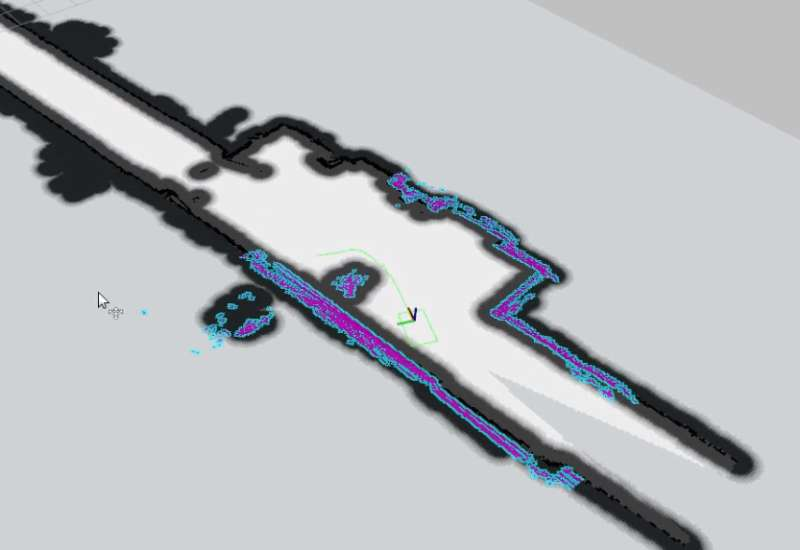
\includegraphics[scale=0.4]{niv.jpg}
	\caption{Navigation show}
\end{figure*}
